%!TEX platex=1
\documentclass[11pt,xcolor=dvipsnames,table,dvipdfmx]{beamer}
\usepackage{amsmath, amssymb}
\usepackage{latexsym}
\usepackage{ascmac}
\usepackage{bm}

%Beamer$B$N@_Dj(B
\usetheme{Boadilla}
%Beamer$B%U%)%s%H@_Dj(B
\usepackage{txfonts} % TX$B%U%)%s%H(B
\usepackage[deluxe]{otf} % $BF|K\8lB?%&%'%$%H2=(B
\renewcommand{\familydefault}{\sfdefault}  % $B1QJ8$r%5%s%;%j%UBN$K(B
\renewcommand{\kanjifamilydefault}{\gtdefault}  % $BF|K\8l$r%4%7%C%/BN$K(B
\usefonttheme{professionalfonts}
\setbeamerfont{alerted text}{series=\bfseries} % Alert$B$rB@;z(B
\setbeamerfont{section in toc}{series=\mdseries} % $BL\<!$OB@;z$K$7$J$$(B
\setbeamerfont{frametitle}{size=\Large} % $B%U%l!<%`%?%$%H%kJ8;z%5%$%:(B
\setbeamerfont{title}{size=\LARGE} % $B%?%$%H%kJ8;z%5%$%:(B
\setbeamerfont{date}{size=\small}  % $BF|IUJ8;z%5%$%:(B

%Beamer$B?'@_Dj(B
\definecolor{UniBlue}{RGB}{0,150,200} 
\definecolor{AlertOrange}{RGB}{255,76,0}
\definecolor{AlmostBlack}{RGB}{38,38,38}
\setbeamercolor{normal text}{fg=AlmostBlack}  % $BK\J8%+%i!<(B
\setbeamercolor{structure}{fg=UniBlue} % $B8+=P$7%+%i!<(B
\setbeamercolor{block title}{fg=UniBlue!50!black} % $B%V%m%C%/ItJ,%?%$%H%k%+%i!<(B
\setbeamercolor{alerted text}{fg=AlertOrange} % \alert $BJ8;z%+%i!<(B
\mode<beamer>{
    \definecolor{BackGroundGray}{RGB}{254,254,254}
    \setbeamercolor{background canvas}{bg=BackGroundGray} % $B%9%i%$%I%b!<%I$N$_GX7J$r$o$:$+$K%0%l!<$K$9$k(B
}

%$B%U%i%C%H%G%6%$%s2=(B
\setbeamertemplate{blocks}[rounded] % Block$B$N1F$r>C$9(B
\useinnertheme{circles} % $B2U>r=q$-$r%7%s%W%k$K(B
\setbeamertemplate{navigation symbols}{} % $B%J%S%2!<%7%g%s%7%s%\%k$r>C$9(B
\setbeamertemplate{footline}[frame number] % $B%U%C%?!<$O%9%i%$%IHV9f$N$_(B

%$B%?%$%H%k%Z!<%8(B
\setbeamertemplate{title page}{%
    \vspace{2.5em}
    {\usebeamerfont{title} \usebeamercolor[fg]{title} \inserttitle \par}
    {\usebeamerfont{subtitle}\usebeamercolor[fg]{subtitle}\insertsubtitle \par}
    \vspace{1.5em}
    \begin{flushright}
        \usebeamerfont{author}\insertauthor\par
        \usebeamerfont{institute}\insertinstitute \par
        \vspace{3em}
        \usebeamerfont{date}\insertdate\par
        \usebeamercolor[fg]{titlegraphic}\inserttitlegraphic
    \end{flushright}
}

% graphicx.sty
\usepackage{graphicx}

%
\def\qed{\hfill $\Box$}

\AtBeginSection[]{
    \frame{\tableofcontents[currentsection, hideallsubsections]} %$BL\<!%9%i%$%I(B
}

%$B%?%$%H%k(B
\title{Monthly Meeting on September}
\author{\textbf{Yuichiro Honda}}
\date{2016/09/09}
\institute{Morita lab. M1}
\begin{document}
\maketitle

\section{Previous work}
\begin{frame}{matroid}
 \begin{block}{definition}
  Let $M = (S, \mathcal{I})$ where $S$ is ground set, and $\mathcal{I}$ is a family satisfying $\mathcal{I} \subseteqq 2^S$. $M$ is called a \alert{matroid} when $\mathcal{I}$ satisfies:
  \begin{align}
   &\emptyset \in \mathcal{I} \\
   &I_1 \subset I_2 , I_2 \in \mathcal{I} \Rightarrow I_1 \in \mathcal{I} \\
   &I_1 , I_2 \in \mathcal{I} , |I_1| < |I_2| \Rightarrow \exists i_2 \in I_2 \setminus I_1 \, ; \; I_1 \cup \{i_2\} \in \mathcal{I}
  \end{align}
 \end{block}
\end{frame}


\begin{frame}{On Disjoint Common Bases in Two Matroids}
 \begin{alertblock}{problem(open)} \it
  input: $M_1 = (S,\,\mathcal{I}_1),\,\,M_2 = (S,\,\mathcal{I}_2)$ : matroids \\
  output: partition of $S$ into common bases of $M_1$ and $M_2$ \\
  \begin{figure}
   \centering
   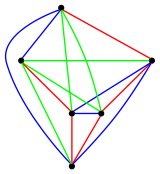
\includegraphics[width=2cm]{partitioned-graph.png}
  \end{figure}
 \end{alertblock}
 \vspace{0.5cm}
 \centering{\large{$\rightarrow$ Can be solved in polynomial time?}}
\end{frame}

\begin{frame}{On Disjoint Common Bases in Two Matroids}
 \begin{figure}
  \centering
  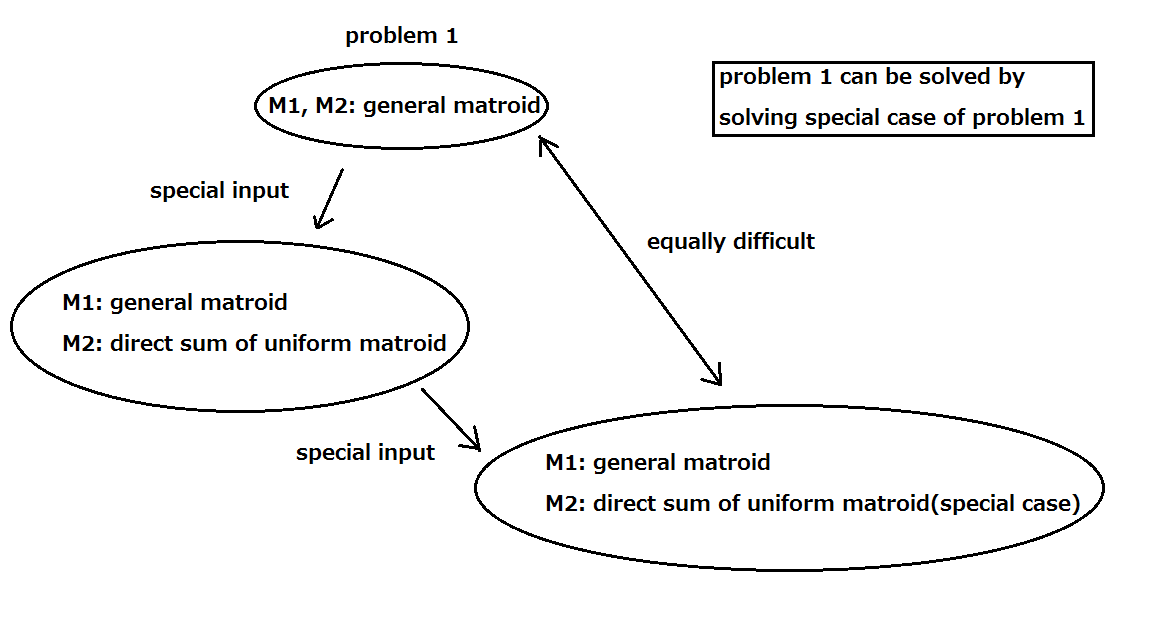
\includegraphics[width=12cm]{problem1.png}
 \end{figure}
\end{frame}


\section{Progress}
\begin{frame}{primitive plan}
\begin{enumerate}
 \item prepare some algorithm to find all common bases
 \item check disjoint combination among them
\end{enumerate}
\end{frame}


\begin{frame}{primitive plan}
\begin{enumerate}
 \item prepare some algorithm to find all common bases
 \item check disjoint combination among them \textcolor{red}{(NP hard?)}
\end{enumerate}
\end{frame}


\begin{frame}{primitive plan}
 Last month, I came across a paper that suggested a method to find all common bases in two matroids in $O(n(n^2 + t)\lambda)$ : \\
 {\it Finding all common bases in two matroids (Fukuda, Namiki 1993)} \\
\end{frame}


\begin{frame}{Hall's theorem}
 $\mathcal{S} = \{S_\lambda\,|\,\,\lambda \in \Lambda\},\,\,S_\lambda$: finite set \\
 \vspace{0.5cm}
 \begin{block}{transversal}
  $X = \{x_\lambda\,|\,\,\lambda \in \Lambda\}$ is \alert{transversal} of $\mathcal{S}$ when $\forall \lambda \in \Lambda \,;\,\,x_\lambda \in S_\lambda$ .
 \end{block}
 \begin{block}{marriage condition}
  $\mathcal{S}$ satisfies the \alert{marriage condition} when \\
  $\forall \mathcal{T} \subseteqq \mathcal{S}\,;\,\,|\mathcal{T}| \leq {\Bigl |}{\displaystyle \bigcup_{A\in \mathcal{T}}A}{\Bigr |}$
 \end{block}
\end{frame}


\begin{frame}{Hall's theorem}
 \begin{block}{Hall's theorem}
  $\mathcal{S} = \{S_\lambda\,|\,\,\lambda \in \Lambda\},\,\,S_\lambda$: finite set \\
  Then, \\ $\mathcal{S}$ satisfies marriage condition $\iff$ $\mathcal{S}$ has transversal
 \end{block}
\end{frame}

\begin{frame}{Hall's theorem}
 \begin{block}{Hall's theorem (graph theory)}
  $G = (X + Y,\,\,E)$ : bipartite graph ($|X| = |Y|$)\\
  $N_G (A)$ : neibourhood of $A \subseteqq X + Y$ \\
  Then, \\ $\forall W \subseteqq X\,;\,\,|W| \leq |N_G (W)|$  $\iff$ $G$ has perfect matching
 \end{block}
\end{frame}


\section{Next step}
\begin{frame}{next month}
 TODO:
 \begin{enumerate}
  \item continue to read a paper: Finding all common bases in two matroids (Fukuda, Namiki 1993)
  \item think about whether $O(n(n^2 + t)\lambda)$ algorithm is applicable
 \end{enumerate}
\end{frame}

\begin{frame}
 \begin{center}
  Thank you for your attention.
 \end{center}
\end{frame}
\end{document}